\documentclass[a4paper]{article}
\usepackage[utf8]{inputenc}
\usepackage{graphicx}
\usepackage{epstopdf}
\usepackage{epsfig}
\usepackage{wrapfig}
\usepackage{subcaption}
\usepackage{float}
\usepackage[english,serbian]{babel}

\begin{document}

\title{Logistička modifikacija Lotka-Voltera modela\\
	\small{Seminarski u okviru kursa\\Osnove matematičkog modeliranja\\Matematički fakultet}
}
\author{Marina Brkić, Nikola Vlahović\\marinabrkic91@gmail.com\\nikola.vlahovic2401@gmail.com}
\date{27. ~maj 2018.}
\maketitle
\abstract{
	Lotka-Voltera nelinearne diferencne jednačine prvog reda 
	se koriste za modeliranje populacija sa predator-plen interakcijom.
	Predstavljamo standardne jednačine i modifikaciju koja uzima u obzir
	ograničen kapacitet staništa.

	Ključne reči: populacija, predator-plen
}
\tableofcontents

\newpage

\section{Uvod}
\label{sec:uvod}

\section{Standardni Lotka-Voltera model}
\label{sec:std_model}
Pretpostavimo da populacija lisica jede samo zečeve i označimo
tu populaciju sa x(t) u vremenu t.
Ako nema zečeva populacija lisica će izumreti, na
osnovu diferencne jednačine x'=-dx, gde je d razlika stope rodjenja i stope umiranja.
Populacija zečeva y(t), bez lisica, će nastaviti da raste na osnovu diferencne jednačine y'=by, gde je b razlika stope rodjenja i stope umiranja.
želimo slučaj kada su obe populacije pozitivne. Za slučaj lisica treba nam dodatna promenljiva
sa desne strane koja će biti pozitivna kada ima zečeva. Tačnije, ta promenljiva treba da bude velika ako su
x(t) ili y(t) veliki. Postoji mnogo načina da se to uradi, a mi ćemo tako što ćemo modifikovati d tako da bude
-d + ey. e je pozitivna konstanta jer su zečevi izvor hrane za lisice. Tada dobijamo da je jednačina za lisice:
		\begin{center}
		$x' = (-a + by)x,   x(0)=x_0$
		\end{center}
Na sličan način dobijamo jednačinu za zečeve, s tim što u ovom slučaju populacija zečeva treba da se smanjuje pa ćemo ubaciti -cx. Dobijamo jednačinu: 
		\begin{center}
		$y' = (c - mx)y,  y(0)=y_0$
		\end{center}
Ove dve jednačine su poznate kao \textbf{Lotka-Voltera sistem diferencnih jednačina}. \\

Rešenje ovog sistema je teško naći i zbog toga se koriste numeričke metode. U broju populacije biće oscilacija.
Ako je populacija zečeva mnogo velika onda će biti mnogo hrane za lisice i populacija će se povećati.
Kako se populacija lisica bude povećavala tako će se broj zečeva smanjivati. A kako se bude smanjivala
količina hrane za lisice, tako će se i populacija lisica smanjivati. Očekivanja su da je savršeni balans populacija
kada se nijedna populacija ne menja. To znači da su  x'=0 i y'=0. Ovo se zove  \textbf{ravnotežno stanje}.
Postoji po jedno pozitivno ravnotežno stanje za obe jednačine, i to su $x=b/c$ iz jednačine za zečeve i $y=d/e$, iz jednačine za lisice.\\ 
Zaključujemo da  graf sa tačkama (x(t),y(t)) mora biti zatvorena kriva.
Da bi ovo videli, razmotrimo funkciju H(x(t),y(t)), gde
je H(x,y)=c $ln(x)$ - mx + a $ln(x)$ - by i x(t) i y(t) zadovoljavaju Lotka-Voltera jednačinu.
Promena vremena se racuna pomoću pravila lanca i to: \\ \\ $H'=H_x x' + H_y y' = (b/x - c)(-d + ey)x + (d/y - e)(b - cx)y = 0$ \\ \\
Tako da  H(x(t),y(t)) mora biti konstanta. Može se pokazati da H(x,y)= constant definiše jednostavnu zatvorenu krivu.

\subsection{Primer u Matlabu}
\label{sub:std_primer}
Da bi rešili ovaj sistem jednačina koristićemo Matlab funkciju ode45. Ova funkcija koristi Runge-Kuta
formule četvrtog i petog stepena za automatsko integrisanje.\\ \\
 Naše jednačine su 
	\begin{center}
		$x' = -ax + bxy$
	\end{center}
	\begin{center}
		$y' =yc - mxy$
	\end{center}
Kada ubacimo vrednosti parametara koje su a=3, b=2, c=1, m=2.5 i jednačine izjednačimo sa 0, dobijamo:
	\begin{center}
		$x'=3x - 2xy = 0$
	\end{center}
	\begin{center}
		$y'=-y + 2.5xy = 0$
	\end{center}
U Matlabu pravimo m fajl $ standard\_equations.m $:
\begin{flushleft}
	$lv\_standard = @(t, state) [$ \\
  	$  a * state(1) - b * state(1) * state(2);$\\
	$    c * state(1) * state(2) - m * state(2)$\\
	$    ];$
	$[ts, ys] = ode45(lv\_standard, [0, 10], [p\_init;g\_init]);$
	$plot\_figures(ts, ys, lv\_standard);$
\end{flushleft}
Fazni dijagram pravimo pomoću m fajla $ plot\_figures.m $:
\begin{flushleft}
	$function [] = plot\_figures(ts, ys, equations)$\\
   	$plot(ts, ys)$\\
   	$legend('plen', 'predator')$\\
   	$figure();$\\
   	$plot(ys(:,1),ys(:,2)); hold on$           \hspace{2cm}\%plot solution in phase plane \\
   	$xlabel('plen'); ylabel('predator')$
\end{flushleft} 

\begin{figure}[H]
    \centering
    \begin{minipage}{0.45\textwidth}
        \centering
        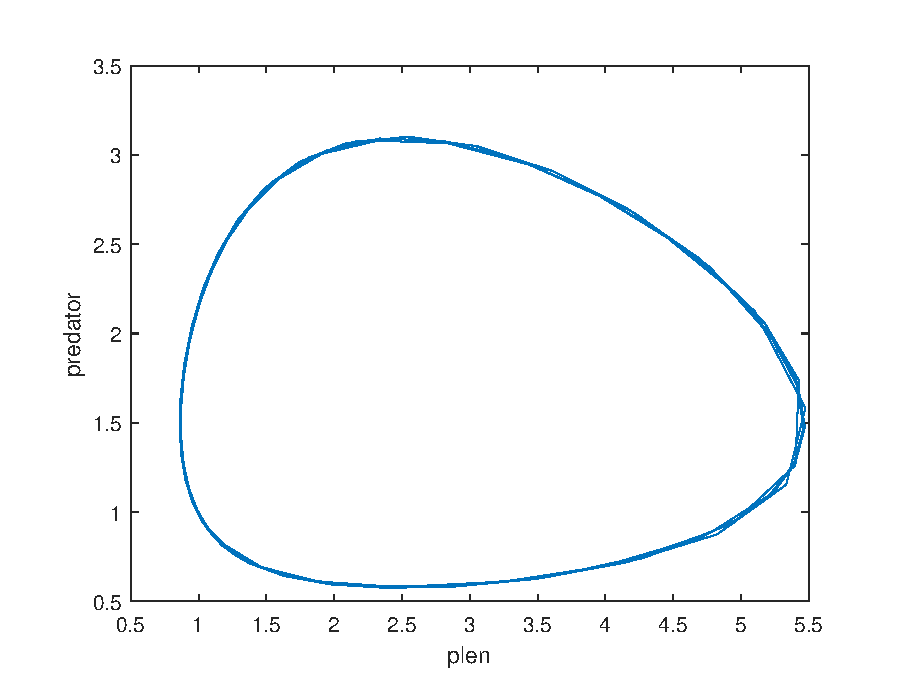
\includegraphics[width=1\textwidth]{images/lotka_voltera_phase} % first figure itself
        \caption{Fazni dijagram standardnog modela}
    \end{minipage}\hfill
    \begin{minipage}{0.45\textwidth}
        \centering
        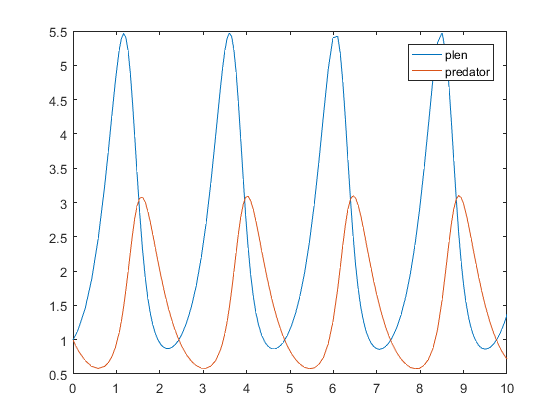
\includegraphics[width=1\textwidth]{images/lotka_voltera_time_plot} % second figure itself
        \caption{Grafik promene populacija kroz vreme za standardni model}
    \end{minipage}
\end{figure}

\section{Logistička modifikacija Lotka-Voltera modela}
\label{sec:log_mod}
Ukoliko je prirodni priraštaj negativan, populacija će eksponencijalno opadati ka nuli,
tj. težiće izumiranju. Ako je prirodni priraštaj pozitivan, populacija će da raste.
Može se videti da je ovaj model realističan sve dok je prirodni priraštaj konstantan.\\
Znamo da na realnom, konačnom staništu populacija ne može neograničeno rasti zbog
ograničenih raspoloživih resursa. Dakle, stanište može da podrži odredjen maksimalan broj
jedinki neke vrste. Označimo taj maksimum sa U. Kada ovaj maksimalni broj živi duže vreme u
nepromenjenom broju jasno je da je priraštaj u toj situaciji jednak nuli. Iskoristivši pretpostavku
da priraštaj linearno zavisi od veličine populacija, belgijski matemaričar Verhulst je predložio model:
	\begin{center}
		$\frac{dN(t)}{dt}=rN (t) (1 - \frac{N (t)}{U})$
	\end{center}
Mi smo iskoristili ovu jednačinu tako što smo zamenili u jednačini za plen deo
formule za priraštaj plena logističkom formulom. Time smo uračunali zavisnost
priraštaja od odnosa veličine populacije i kapaciteta staništa.\\

\subsection{Primer u Matlabu}
\label{sub:log_mod_matlab}

Fazni dijagram za modifikaciju modela formiramo pomoću m fajla $ logistic\_equations.m $, kada
trava ne može da ishrani više od U zečeva, gde nam je U parametar u logističkom modelu:

\begin{flushleft}
	$lv\_logistic = @ (t, state) [ $\\
	$a * state(1) * ( 1 - (state(1))/u) - b * state(1) * state(2);$\\
	$c * state(1) * state(2) - m * state(2)$\\
	$];$\\
	$[ts, ys] = ode45(lv\_logistic, [0, 15], [p\_init;g\_init]);$\\
	$plot\_figures(ts, ys, lv_logistic); $
\end{flushleft}
 

\begin{figure}[H]
    \centering
    \begin{minipage}{0.45\textwidth}
        \centering
        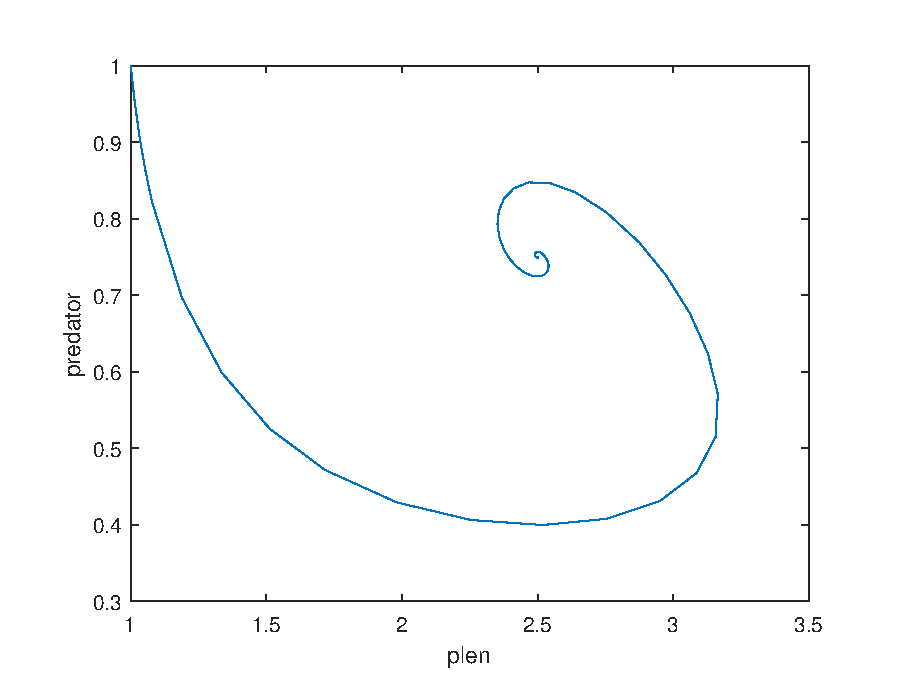
\includegraphics[width=1\textwidth]{images/lotka_voltera_logistic_phase} % first figure itself
        \caption{Fazni dijagram za U=5}
    \end{minipage}\hfill
    \begin{minipage}{0.45\textwidth}
        \centering
        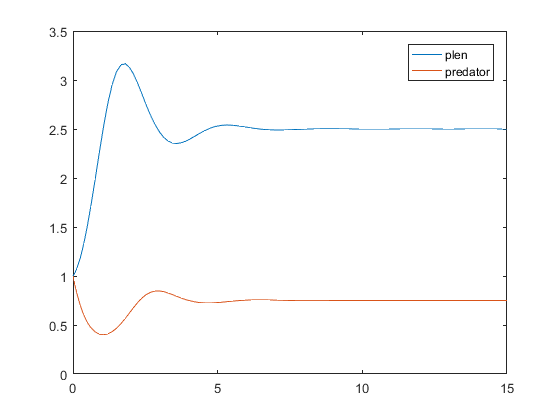
\includegraphics[width=1\textwidth]{images/lotka_voltera_logistic_time_plot} % second figure itself
        \caption{Promena populacija za U=5}
    \end{minipage}
\end{figure}


\subsection{Stanište sa vrlo ograničenim kapacitetom}
\label{sub:log_mod_ogr}

\begin{figure}[H]
    \centering
    \begin{minipage}{0.45\textwidth}
        \centering
        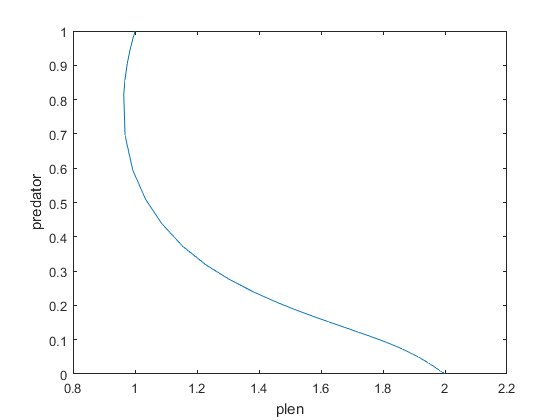
\includegraphics[width=1\textwidth]{images/lv_low_u_phase} % first figure itself
        \caption{Fazni dijagram za U=2}
    \end{minipage}\hfill
    \begin{minipage}{0.45\textwidth}
        \centering
        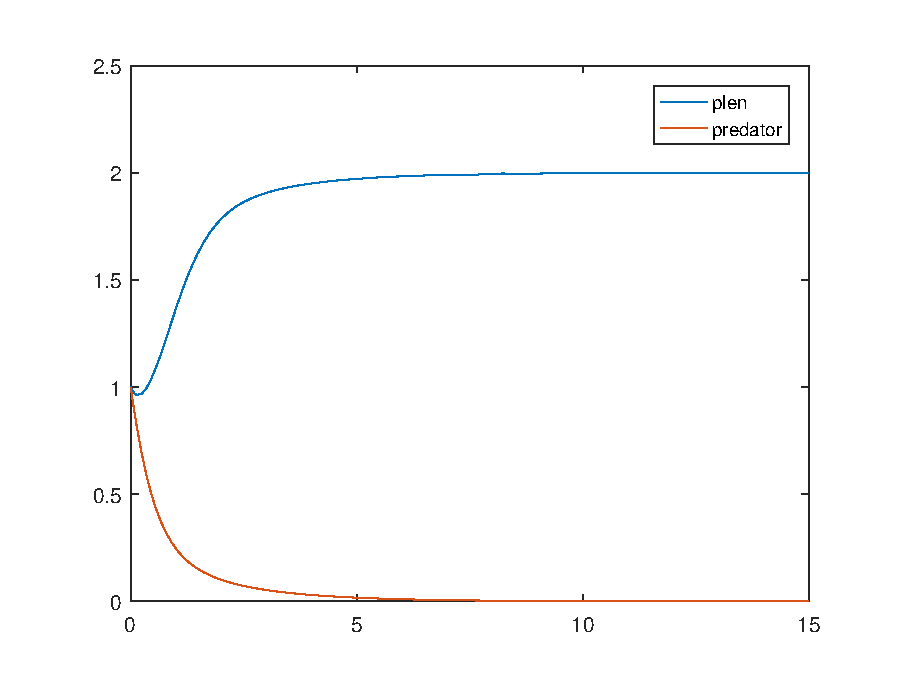
\includegraphics[width=1\textwidth]{images/lv_low_u_time} % second figure itself
        \caption{Promena populacija za U=2}
    \end{minipage}
\end{figure}


\end{document}